% Setup our document
\documentclass[12pt, a4paper]{article}
\usepackage{tikz}
\usepackage{transparent}

% Start our document content
\begin{document}
\title{Hello Tex}
\author{Arthur De Witte}
\maketitle

\tableofcontents

% Create a section
\section{Why Tex?}
Soo, LaTeX has a few advantages, one of them is that you can easily implement math.

For example \(4^5\) or \(e^{5*\frac{6}{\pi}}\)

\section{Drawing}

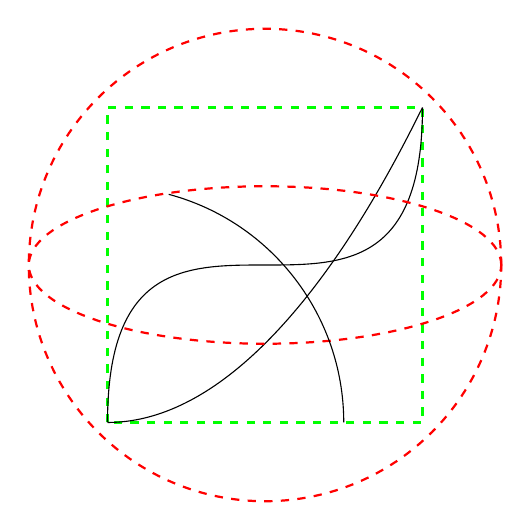
\begin{tikzpicture}

  % \draw (0, 0) -- (4, 0) -- (4, 4) -- (0, 4) -- cycle;
  \draw[green, thick, dashed] (0, 0) rectangle (4, 4);
  \draw (0, 0) parabola (4, 4);
  \draw (0, 0) .. controls (0, 4) and (4, 0) .. (4, 4);

  \draw[red, thick, dashed] (2, 2) circle (3cm);
  \draw[red, thick, dashed] (2, 2) ellipse (3cm and 1cm);

  \draw (3, 0) arc (0:75:3cm);

\end{tikzpicture}

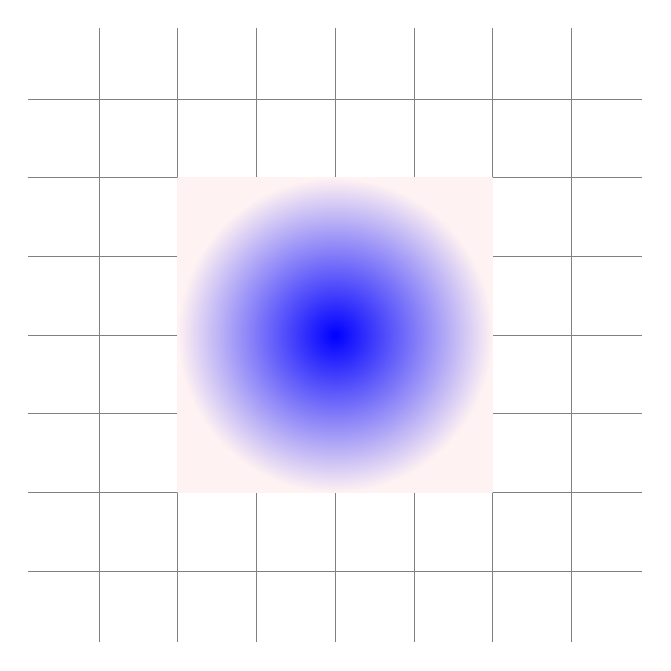
\begin{tikzpicture}

  \draw[step=1cm, gray, very thin] (-1.9, -1.9) grid (5.9, 5.9);
  % \fill[blue!40!white, draw=black] (0, 0) rectangle (4, 4);
  % \shade[top color=blue, bottom color=red] (0, 0) rectangle (4, 4);
  \shade[inner color=blue, outer color={white!95!red}] (0, 0) rectangle (4, 4);

\end{tikzpicture}

\end{document}
